\documentclass[11pt]{article}
\usepackage[margin=1.0in]{geometry}
\usepackage{lastpage}
\usepackage{mathtools}
\usepackage{graphicx}
\usepackage{float}
\usepackage[font=small]{caption}
\usepackage{color}
\usepackage{fancyhdr}
%\usepackage{soul} %for striking out text
%\usepackage{arydshln} % for dotted line on truth table
\usepackage{tikz} % graphics stuff
\usepackage{caption}
\usepackage{gensymb}
\usepackage{booktabs}
\usepackage{listings}
\usepackage{fancyvrb}
%\usepackage{subcaption} % used to horizontally tile figures
%\usepackage{listings}
\pagestyle{fancy}
\fancyhead{}
\fancyfoot{}


\newcommand{\ClassNameS}{CMPE-630}
\newcommand{\ClassNameL}{Digital Integrated Circuit Design}
\newcommand{\ExerciseName}{Final Project}
\newcommand{\SubTitle}{Multiply and Accumulate (MAC) Datapath Unit Design}
\newcommand{\Arthur}{Brandon Key \& Chris Guarini}
\newcommand{\DueDate}{9 Dec 2019}

\fancyhead[L]{\ClassNameS}
\fancyhead[R]{\ExerciseName}

\fancyfoot[L]{\Arthur}
\fancyfoot[C]{\DueDate}
\fancyfoot[R]{\thepage \space of \pageref{LastPage}}

\setlength{\parindent}{0em}
\setlength{\parskip}{1em}

\linespread{1.0}
% where value determine line spacing.
% 1.0	single spacing
% 1.3	one-and-a-half spacing
% 1.6	double spacing

\definecolor{mygreen}{rgb}{0,0.6,0}
\definecolor{mygray}{rgb}{0.5,0.5,0.5}
\definecolor{mymauve}{rgb}{0.58,0,0.82}

\lstset{ 
	backgroundcolor=\color{white},   % choose the background color; you must add \usepackage{color} or \usepackage{xcolor}; should come as last argument
	basicstyle=\footnotesize,        % the size of the fonts that are used for the code
	breakatwhitespace=false,         % sets if automatic breaks should only happen at whitespace
	breaklines=true,                 % sets automatic line breaking
	captionpos=t,                    % sets the caption-position to bottom
	commentstyle=\color{mygreen},    % comment style
	deletekeywords={},               % if you want to delete keywords from the given language
	escapeinside={\%*}{*)},          % if you want to add LaTeX within your code
	extendedchars=false,             % lets you use non-ASCII characters; for 8-bits encodings only, does not work with UTF-8
	firstnumber=0,                   % start line enumeration with line 1000
	frame=single,                    % adds a frame around the code
	keepspaces=true,                 % keeps spaces in text, useful for keeping indentation of code (possibly needs columns=flexible)
	keywordstyle=\color{blue},       % keyword style
	language=VHDL,                   % the language of the code
	morekeywords={},                 % if you want to add more keywords to the set
	numbers=left,                    % where to put the line-numbers; possible values are (none, left, right)
	numbersep=5pt,                   % how far the line-numbers are from the code
	numberstyle=\tiny\color{mygray}, % the style that is used for the line-numbers
	rulecolor=\color{black},         % if not set, the frame-color may be changed on line-breaks within not-black text (e.g. comments (green here))
	showspaces=false,                % show spaces everywhere adding particular underscores; it overrides 'showstringspaces'
	showstringspaces=false,          % underline spaces within strings only
	showtabs=false,                  % show tabs within strings adding particular underscores
	stepnumber=5,                    % the step between two line-numbers. If it's 1, each line will be numbered
	stringstyle=\color{mymauve},     % string literal style
	tabsize=4, 	                     % sets default tabsize to 2 spaces
	title=\lstname                   % show the filename of files included with \lstinputlisting; also try caption instead of title
}

\begin{document}\thispagestyle{empty}

%
% cover page
%

\vspace*{2 cm}

\begin{center}
\bf{\ClassNameS \space \ClassNameL\\
    \ExerciseName\\
\vspace{0.25 cm}
\SubTitle
}
\end{center}

\vspace{4 cm}

\begin{flushright}
Brandon Key\\
Chris Guarini\\
Performed: 9 Dec 2019\\
Submitted: \DueDate\\
\vspace{0.5 cm}
Instructor: Dr. Amlan Ganguly\\
TAs: Abhishek Vashist\\
Andrew Fountain\\
Piers Kwan\\
\vspace{0.5 cm}
\end{flushright}

\vspace{2 cm}
\indent By submitting this report, you attest that you neither have given nor have received any assistance (including writing, collecting data, plotting figures, tables or graphs, or using previous student reports as a reference), and you further acknowledge that giving or receiving such assistance will result in a failing grade for this course.

\vspace{1 cm}

Brandon Key:   \rule{13cm}{.1pt}\\
\vspace{1 cm}

Chris Guarini:   \rule{13cm}{.1pt}

\newpage
\tableofcontents
\newpage

\section{Abstract}

	
	

\section{Design Methodology and Theory}

	A cornerstone of IC design is the ability to create large, complex designs from smaller more manageable parts. The project outlined in this exercise calls for the design, testing and layout of a multiply and accumulate (MAC) unit, which takes two 16-bit inputs, multiplies them together, adds them to the value stored in a register, and then stores that output back into the register. The final component should contain a built in self test (BIST) that verifies the functionality of the MAC.
	
	The MAC is composed of a carry-save multiplier, ripple carry full-adder, and parallel register. The BIST is implemented through the use of an LFSR for the inputs, an MISR for the output, and a test controller which controls the timing and sets the test passed and test complete outputs. A full diagram of the MAC with BIST can be seen in Figure \ref{fig:full-project-block}.
	
	\begin{figure}[H]
		\centering
		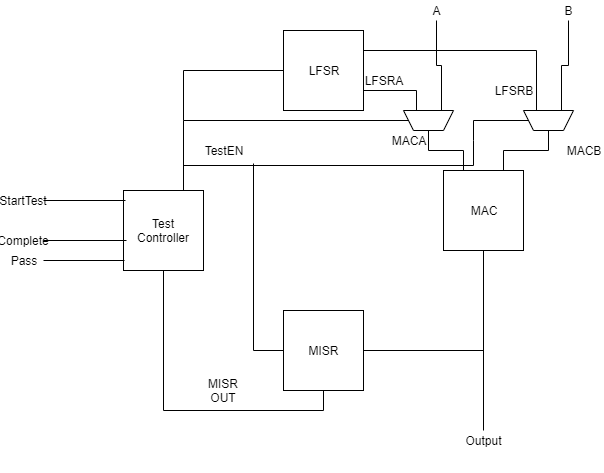
\includegraphics[width=0.7\linewidth]{Pictures/Full-Project-Block}
		\caption{High Level Block Diagram of the MAC with BIST}
		\label{fig:full-project-block}
	\end{figure}


	\subsection{User Operation}
		The full MAC and BIST design has a total of six inputs and three outputs, which are shown in Table \ref{tab:Inputs} and Table \ref{tab:Outputs} respectively. All inputs and outputs of the MAC are clocked, so a clk signal is required for operation. To enable the writing to register, WE must be high for both MAC and BIST functionality. This allows for initialization of input values without it writing to the registers, and for the ability to hold what value the registers contain without changing the inputs. 
		
		In order to run the MAC in its functional mode, WE must be high, reset and StartTest must be low. Once these requirements are met, the values of inputs A and B will be multiplied together and accumulated into the registers. The output RegOut will contain the current value in the register.
		
		To run the BIST, the component must first be reset for a total of three clock cycles during initializing. This can be achieved by holding reset low during initialization. Afterwords, reset, WE and StartTest should be high. The BIST runs for a total of 1000 clock cycles, during which the outputs Pass and Complete will be low. When Complete goes high the BIST is over and Pass will contain whether the test passed or not.
		
		\begin{table}[H]
			\centering
			\caption{Inputs of the MAC}
			\label{tab:Inputs}
			\begin{tabular}{|ccc|}
				\hline
				\textbf{}   \textbf{Input}      & \textbf{Function} &  \textbf{Size (Bits)} \\
				\hline
				\textbf{A}  & Input 1 & N/2          \\
				\textbf{B}  & Input 2 & N/2            \\ 
				\textbf{clk}  & Clock Signal & 1        \\ 
				\textbf{WE}  & Write Enable & 1           \\ 
				\textbf{reset}  & Active Low Reset & 1           \\ 
				\textbf{StartTest}  & Enable BIST & 1           \\ 
				\hline                     
			\end{tabular}
		\end{table}
		
		\begin{table}[H]
			\centering
			\caption{Outputs of the MAC}
			\label{tab:Outputs}
			\begin{tabular}{|ccc|}
				\hline
				\textbf{}   \textbf{Output}      & \textbf{Function} &  \textbf{Size (Bits)} \\
				\hline
				\textbf{RegOut}  & Output of the MAC & N          \\
				\textbf{Pass}  & BIST Pass Flag & 1            \\ 
				\textbf{Complete}  & BIST Complete Flag & 1        \\ 
				\hline                     
			\end{tabular}
		\end{table}
	

	\subsection{Adder}
	
		The adder used in this design is an N-bit ripple carry adder which accepts input from the outputs of the multiplier and accumulation register. A ripple carry adder is composed of a series of N full adders, where the carry-out of the previous full adder is fed into the carry-in of the next full adder, as shown in Figure \ref{fig:ripple-carry-adder}.
		
		\begin{figure}[H]
			\centering
			\includegraphics[width=0.6\textwidth,height=\dimexpr\textheight-4\baselineskip-\abovecaptionskip-\belowcaptionskip\relax,keepaspectratio]{"Pictures/Ripple Carry Adder"}
			\caption{Ripple Carry Adder}
			\label{fig:ripple-carry-adder}
		\end{figure}
		
		The code in Figure \ref{code:nBitAdder} shows one of the generate statements used to create the nBitAdder from full adder components. The uses VHDL generate statements to generate N-2 full adders that take their carry-in bit from the previous full adder and send their carry out to the next full adder through the internal signal carray. The first and last full adder in the series are generated differently, as the first full adder's carry-in is hard coded to 0 and the last full adder's carry-out is an output. The full code of the nBitAdder is available in Listing \ref{lst:nBitAdder-vhd} of the appendix.
		
		\begin{figure}[H]
		\centering
		\begin{verbatim}
            i_mid : if (i /= 0) and (i /= (n-1)) generate
                adder : full_adder port map(
                    A => A(i),
                    B => B(i),
                    Cin => c_array(i-1),
                    Sum => Y(i),
                    Cout => c_array(i)
                );
            end generate i_mid;
        \end{verbatim}
        \caption{nBitAdder Code Snippet} 
    	\label{code:nBitAdder} 
    	\end{figure}
	
		\begin{figure}[H] 
			\centering 
			\includegraphics[width=\textwidth,height=\dimexpr\textheight-4\baselineskip-\abovecaptionskip-\belowcaptionskip\relax,keepaspectratio]{"Pictures/nBitAdder Schematic Page 1"}
			\caption{nBitAdder Schematic Page 1} 
			\label{fig:nBitAdder-Schematic-Page-1} 
		\end{figure}
		
		
		\begin{figure}[H] 
			\centering 
			\includegraphics[width=\textwidth,height=\dimexpr\textheight-4\baselineskip-\abovecaptionskip-\belowcaptionskip\relax,keepaspectratio]{"Pictures/nBitAdder Schematic Page 2"}
			\caption{nBitAdder Schematic Page 2} 
			\label{fig:nBitAdder-Schematic-Page-2} 
		\end{figure}
	
	\subsection{Multiplier}
	
	The MAC includes a carry-save multiplier component in order to multiply the two inputs together. A carry-save multiplier works as shown in Figure \ref{fig:multiplier-block-dia}, where full adders are arranged in a 2d array where each row is N/2 adders long and offset by 1.
		
		\begin{figure}[H]
			\centering
			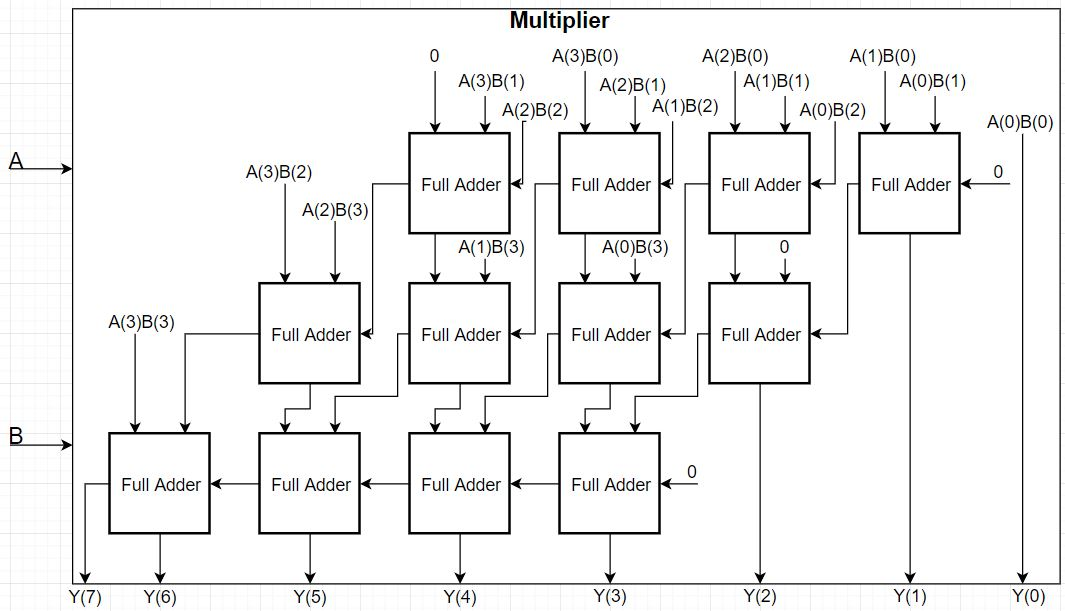
\includegraphics[width=\textwidth,height=\dimexpr\textheight-4\baselineskip-\abovecaptionskip-\belowcaptionskip\relax,keepaspectratio]{Pictures/Multiplier}
			\caption{Carry-Save Multiplier Block Diagram}
			\label{fig:multiplier-block-dia}
		\end{figure}
		
	The full VHDL code for the multiplier is found in Listing \ref{lst:Multiplier-vhd}. The code takes advantage of VHDL generate statements to generate the four different connections a full adder could have in a carry-save multiplier. The first fill adder of each row, the last full adder of the first row, the last full adder of every other row, and all other full adders.
	
	Figures \ref{fig:Multiplier-Schematic-Page-1} and \ref{fig:Multiplier-Schematic-Page-2} show both pages of the multiplier schematic. These schematics were generated from the VHDL code in \ref{lst:Multiplier-vhd} using Spectrum scripts to create a Verilog file that was then imported into Pyxis.
	
	
		\begin{figure}[H] 
			\centering 
			\includegraphics[width=\textwidth,height=\dimexpr\textheight-4\baselineskip-\abovecaptionskip-\belowcaptionskip\relax,keepaspectratio]{"Pictures/Multiplier Schematic Page 1"}
			\caption{Multiplier Schematic Page 1} 
			\label{fig:Multiplier-Schematic-Page-1} 
		\end{figure}
		
		
		\begin{figure}[H] 
			\centering 
			\includegraphics[width=\textwidth,height=\dimexpr\textheight-4\baselineskip-\abovecaptionskip-\belowcaptionskip\relax,keepaspectratio]{"Pictures/Multiplier Schematic Page 2"}
			\caption{Multiplier Schematic Page 2} 
			\label{fig:Multiplier-Schematic-Page-2} 
		\end{figure}
	
	\subsection{16-Bit Register}
	
	Two 16-bit parallel registers are used to clock the two inputs to the multiplier. The VHDL architecture for the register can be seen in Figure \ref{code:nBitRegister_16}, which shows that the register has an active low reset, and when WE is high will take new input. Otherwise the register holds its previous value.
	
	\begin{figure}[H]
		\centering
		\begin{verbatim}
            architecture behav of nBitRegister_16 is
            begin
                output_proc : process (clk, Reset) begin
                    if Reset = '0' then
                        Y <= (others => '0');
                    elsif clk'event and clk = '1' then
                        if WE = '1' then
                            Y <= nBitIn;
                        end if;
                    end if;
                end process output_proc;
            end behav;
        \end{verbatim}
        \caption{16-Bit Register Code Snippet} 
    	\label{code:nBitRegister_16} 
    \end{figure}
    
    Figure \ref{fig:nBitRegister-16-Bit-Schematic} shows the schematic for the 16-bit register, which provides some insight into how a parallel register is made. There are 16 flip-flops which are connected to their respective input bits, the inverse of the reset signal, a write enable signal, and the clock. Their outputs are connected to the respective output bit.

		\begin{figure}[H] 
			\centering 
			\includegraphics[width=\textwidth,height=\dimexpr\textheight-4\baselineskip-\abovecaptionskip-\belowcaptionskip\relax,keepaspectratio]{"Pictures/nBitRegister 16-Bit Schematic"}
			\caption{16 Bit Register Schematic} 
			\label{fig:nBitRegister-16-Bit-Schematic} 
		\end{figure}

	\subsection{32-Bit Register}
		
		A 32-bit parallel register is used as the accumulator in the MAC component. The accumulator register if functionally the same as the 16-bit register above, as they are generated from the same generic VHDL code, just with different values for N.
		
		The code in Figure \ref{code:nBitRegister_32} shows the code used to generate the 32-bit register, which is identical to the 16-bit register in all but name. The schematic below in Figure \ref{fig:nBitRegister-32-Bit-Schematic} shows how the 32-bit register is functionally identical to the 16-bit register, just with double the amount of flip-flops and logic.
		
		\begin{figure}[H]
		\centering
		\begin{verbatim}
        architecture behav of nBitRegister_32 is
        begin
            output_proc : process (clk, Reset) begin
                if Reset = '0' then
                    Y <= (others => '0');
                elsif clk'event and clk = '1' then
                    if WE = '1' then
                        Y <= nBitIn;
                    end if;
                end if;
            end process output_proc;
        end behav;
        \end{verbatim}
        \caption{32-Bit Register Code Snippet} 
    	\label{code:nBitRegister_32} 
    \end{figure}
	
		\begin{figure}[H] 
			\centering 
			\includegraphics[width=\textwidth,height=\dimexpr\textheight-4\baselineskip-\abovecaptionskip-\belowcaptionskip\relax,keepaspectratio]{"Pictures/nBitRegister 32-Bit Schematic"}
			\caption{32 Bit Register Schematic} 
			\label{fig:nBitRegister-32-Bit-Schematic} 
		\end{figure}
	
	\subsection{MAC}
		The MAC component takes two N/2 bit inputs, A and B. These inputs are multiplied together using a carry-save multiplier and added together with the value in the register using a ripple carry adder. This value is then stored back into the register where it becomes the N bit output RegOut. The block diagram for this logic is in Figure \ref{fig:MAC-block}.
	
		\begin{figure}[H] 
			\centering 
			\includegraphics[width=\textwidth,height=\dimexpr\textheight-4\baselineskip-\abovecaptionskip-\belowcaptionskip\relax,keepaspectratio]{"Pictures/MAC-block"}
			\caption{MAC block} 
			\label{fig:MAC-block} 
		\end{figure}
		
		A snippet of the VHDL used to structurally create the MAC is shown in Figure \ref{code:MAC}, while the full code is available in Listing \ref{lst:MAC-vhd} of the appendix. The code is a fairly straight forward structural representation of the MAC, using 7 internal signals to map the components together and to the inputs and outputs. The code creates a 32-bit MAC with two 16-bit inputs
		
		
		\begin{figure}[H]
			\centering
			\begin{verbatim}
	        signal MultA,MultB : STD_LOGIC_VECTOR((N/2)-1 downto 0);
	        signal Product : STD_LOGIC_VECTOR(N-1 downto 0);
	        signal adderA, adderB, adderOut : STD_LOGIC_VECTOR(N-1 downto 0);
	        signal cout : STD_LOGIC;
	    
	        begin
	        
	            RegMultInA : nBitRegister_16
	                generic map( N => 16)
	                port map(nBitIn => A,
	                    WE => '1', clk => clk, Reset => reset, 
	                    Y => MultA
	                );
	        		  
	        	 RegMultInB : nBitRegister_16
	        	  generic map( N => 16)
	        	  port map(nBitIn => B,
	        			WE => '1', clk => clk, Reset => reset, 
	        			Y=> MultB
	        	  );
	        	
	            MULT1 : Multiplier
	                generic map( N => 32)
	                port map(A => MultA, B => MultB, Product => Product);
	        
	            RegMultOut : nBitRegister_32
	                generic map( N => 32)
	                port map(nBitIn => Product, WE => '1', Reset => reset, clk => clk, Y => adderB);
	        
	            BigBoyReg : nBitRegister_32
	                generic map( N => 32)
	                port map(nBitIn => adderOut, WE => WE, Reset => reset, clk => clk, Y => adderA);
	        
	            ADD1 : nBitAdder
	                generic map ( N => 32)
	                port map( A => adderA, B => adderB, Y => adderOut, CB => cout);
	        		  
	        	RegOut <= adderA;
	        end Behavioral;
	
	        \end{verbatim}
	        \caption{MAC Code Snippet} 
	    	\label{code:MAC} 
	    \end{figure}
    
	    A VHDL test bench verifying the functionality of the MAC is shown in Figure \ref{fig:MAC-16bit-Test-Bench}. ModelSim was used to simulate this waveform using the stimulus code shown in Figure \ref{code:MAC-tb}. This code starts with an input of 2 and 2, which are multiplied and accumulated. The code then changes to inputs of 2 and 4 after 300 ns.
		
		\begin{figure}[H] 
			\centering 
			\includegraphics[width=\textwidth,height=\dimexpr\textheight-4\baselineskip-\abovecaptionskip-\belowcaptionskip\relax,keepaspectratio]{"Pictures/MAC-Test-Bench-Cropped"}
			\caption{MAC Functional Test Bench} 
			\label{fig:MAC-16bit-Test-Bench} 
		\end{figure}
		
		\begin{figure}[H]
		\centering
		\begin{verbatim}
	        stimulus: process
	        begin
	
	            WE <= '1';
	            reset <= '1';
	            A <= "0000000000000010";
	            B <= "0000000000000010";
	            wait for 300 ns;
	            
	            A <= "0000000000000010";
	            B <= "0000000000000100";
	            wait;
	            
	        end process;
	
	        \end{verbatim}
	        \caption{MAC Test Bench Stimulus Code Snippet} 
	    	\label{code:MAC-tb} 
	    \end{figure}

	
	
	\subsection{Mux}
		In order to implement the BIST functionality of the IC, two 16-bit multiplexers are required on each input into the multiplier's input registers. the multiplexers select whether the input should be from the LFSR or the MAC's input. Figure \ref{code:MUX} shows the code used to create the MUX, which uses a data-flow architecture and a process to select the correct input.
		
		\begin{figure}[H]
		\centering
		\begin{verbatim}
	        architecture  Dataflow  of  nBitMux_2to1  is
	            begin
	                --Mux process
	                the_proc : process (sel, A, B) begin
	                    case sel is 
	                        when '0' =>
	                            Y <= A;
	                        when others =>
	                            Y <= B;
	                    end case;
	                end process the_proc;
	        
	        end  Dataflow;
	
     	\end{verbatim}
     	\caption{MAC Test Bench Stimulus Code Snippet} 
   		\label{code:MUX} 
	    \end{figure}
	    
	    Figure \ref{fig:nBitMux-2to1-Schematic} shows the schematic of the 16-bit MUX. The schematic is 16 gdk MUX 2 to 1 gates in parallel.
	
		\begin{figure}[H] 
			\centering 
			\includegraphics[width=\textwidth,height=\dimexpr\textheight-4\baselineskip-\abovecaptionskip-\belowcaptionskip\relax,keepaspectratio]{"Pictures/nBitMux_2to1 Schematic"}
			\caption{nBitMux 2to1 Schematic} 
			\label{fig:nBitMux-2to1-Schematic} 
		\end{figure}
	
	\subsection{LFSR}
	
		An LFSR is a predictably random number generator with known pattern depending on what the seed is. For the BIST functionality of the IC, a 32-bit LFSR is used to generate the two inputs, with the top 16 bits going to input A and the bottom 16 bits going to input B. The 32-bit LFSR has taps at bit 19, 24 and 25 along with an input seed of 0x00BC614E, or 12345678 in decimal. The inner workings of an 8-bit LFSR can be seen in Figure \ref{fig:lfsr-block}. The register takes the seed and continuously shifts it through the different flip-flops, with a tap on certain bits using XOR gates which randomizes the output.
		
		\begin{figure}[H]
			\centering
			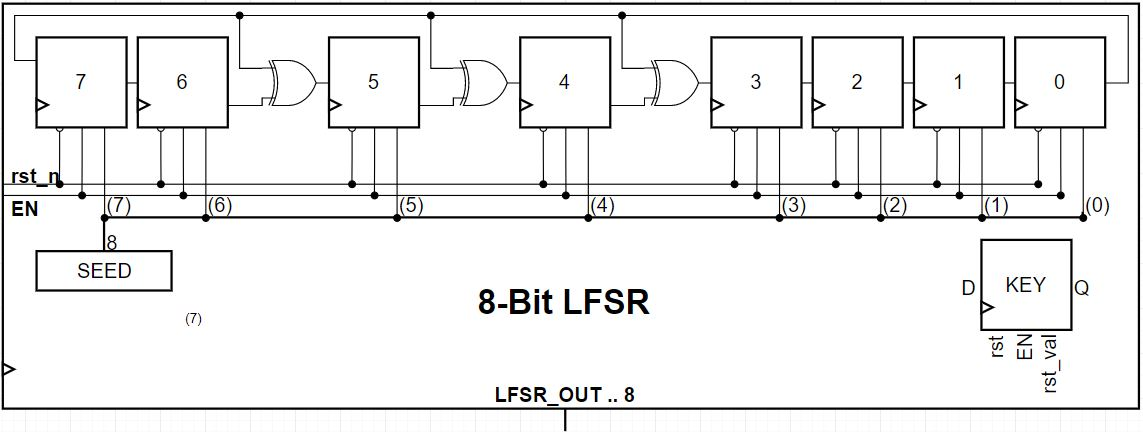
\includegraphics[width=\textwidth,height=\dimexpr\textheight-4\baselineskip-\abovecaptionskip-\belowcaptionskip\relax,keepaspectratio]{Pictures/LFSR}
			\caption{8-Bit Linear Feedback Shift Register}
			\label{fig:lfsr-block}
		\end{figure}
	
	\subsection{MISR}
	
		The MISR is used by the BIST to take the output of the MAC and turns it into a 32-bit signature. The signature is then compared to the one in the test controller to see if the BIST has passed. The purpose of this rather than just comparing the actual output is that the signature takes into account when the output occurred and the previous inputs. This means that no two signatures will be the same, but they are predictably random. Figure \ref{fig:misr-block} is a diagram of an 8-bit MISR as an example. The MISR used in the final design has taps that match the LFSR (19, 24 and 25).  
	
	
		\begin{figure}[H]
			\centering
			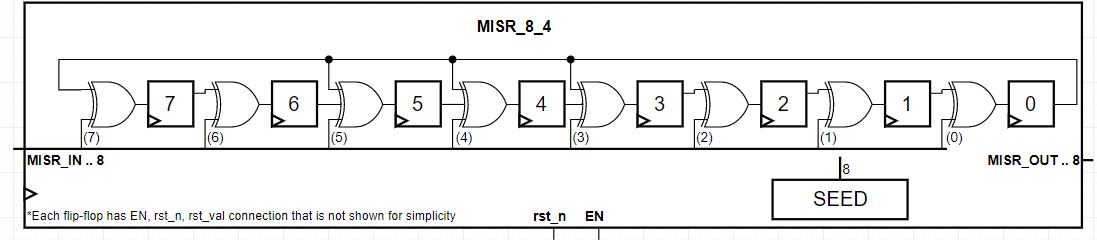
\includegraphics[width=\textwidth,height=\dimexpr\textheight-4\baselineskip-\abovecaptionskip-\belowcaptionskip\relax,keepaspectratio]{Pictures/MISR}
			\caption{Multiple Input Shift Register}
			\label{fig:misr-block}
		\end{figure}
	
	\subsection{BIST}
	
		The test controller used to implement BIST compares the signature of the MISR to an expected signature that would occur after 1000 clock cycles. This is to make sure that the MAC is thoroughly tested with as many inputs as possible. The signature that the controller is looking for is 0x8C9781E6. The waveform in Figure \ref{fig:BIST-Test-Bench} shows how that signature is seen on the 1000 clock cycle, which causes the Complete and Pass outputs to go high, as the BIST completed successfully.
	
		\begin{figure}[H] 
			\centering 
			\includegraphics[width=\textwidth,height=\dimexpr\textheight-4\baselineskip-\abovecaptionskip-\belowcaptionskip\relax,keepaspectratio]{"Pictures/BIST-Test-Bench"}
			\caption{BIST Test Bench} 
			\label{fig:BIST-Test-Bench} 
		\end{figure}
	
	\subsection{Schematic}
	
		The schematics for the MAC with BIST are shown in Figures \ref{fig:Full-Schematic-Page-1} through \ref{fig:Full-Schematic-Page-28}, which is twenty-eight sheets. These sheets were generated using the VHDL code in Listing \ref{lst:ProjectWrapper-vhd} of the appendix, which defines the project structurally. Verilog code was generated from the VHDL using the Leonardo script in Listing \ref{lst:ProjectWrapper-script}, which was then import into Pyxis to generate the schematics.
		
		
		\begin{figure}[H] 
			\centering 
			\includegraphics[width=\textwidth,height=\dimexpr\textheight-4\baselineskip-\abovecaptionskip-\belowcaptionskip\relax,keepaspectratio]{"Pictures/Full Schematic Page 1"}
			\caption{Full Schematic Page 1} 
			\label{fig:Full-Schematic-Page-1} 
		\end{figure}
	
		\begin{figure}[H] 
			\centering 
			\includegraphics[width=\textwidth,height=\dimexpr\textheight-4\baselineskip-\abovecaptionskip-\belowcaptionskip\relax,keepaspectratio]{"Pictures/Full Schematic Page 2"}
			\caption{Full Schematic Page 2} 
			\label{fig:Full-Schematic-Page-2} 
		\end{figure}
	
		\begin{figure}[H] 
			\centering 
			\includegraphics[width=\textwidth,height=\dimexpr\textheight-4\baselineskip-\abovecaptionskip-\belowcaptionskip\relax,keepaspectratio]{"Pictures/Full Schematic Page 3"}
			\caption{Full Schematic Page 3} 
			\label{fig:Full-Schematic-Page-3} 
		\end{figure}
		
		
		\begin{figure}[H] 
			\centering 
			\includegraphics[width=\textwidth,height=\dimexpr\textheight-4\baselineskip-\abovecaptionskip-\belowcaptionskip\relax,keepaspectratio]{"Pictures/Full Schematic Page 4"}
			\caption{Full Schematic Page 4} 
			\label{fig:Full-Schematic-Page-4} 
		\end{figure}
		
		
		\begin{figure}[H] 
			\centering 
			\includegraphics[width=\textwidth,height=\dimexpr\textheight-4\baselineskip-\abovecaptionskip-\belowcaptionskip\relax,keepaspectratio]{"Pictures/Full Schematic Page 5"}
			\caption{Full Schematic Page 5} 
			\label{fig:Full-Schematic-Page-5} 
		\end{figure}
		
		
		\begin{figure}[H] 
			\centering 
			\includegraphics[width=\textwidth,height=\dimexpr\textheight-4\baselineskip-\abovecaptionskip-\belowcaptionskip\relax,keepaspectratio]{"Pictures/Full Schematic Page 6"}
			\caption{Full Schematic Page 6} 
			\label{fig:Full-Schematic-Page-6} 
		\end{figure}
		
		
		\begin{figure}[H] 
			\centering 
			\includegraphics[width=\textwidth,height=\dimexpr\textheight-4\baselineskip-\abovecaptionskip-\belowcaptionskip\relax,keepaspectratio]{"Pictures/Full Schematic Page 7"}
			\caption{Full Schematic Page 7} 
			\label{fig:Full-Schematic-Page-7} 
		\end{figure}
		
		
		\begin{figure}[H] 
			\centering 
			\includegraphics[width=\textwidth,height=\dimexpr\textheight-4\baselineskip-\abovecaptionskip-\belowcaptionskip\relax,keepaspectratio]{"Pictures/Full Schematic Page 8"}
			\caption{Full Schematic Page 8} 
			\label{fig:Full-Schematic-Page-8} 
		\end{figure}
		
		
		\begin{figure}[H] 
			\centering 
			\includegraphics[width=\textwidth,height=\dimexpr\textheight-4\baselineskip-\abovecaptionskip-\belowcaptionskip\relax,keepaspectratio]{"Pictures/Full Schematic Page 9"}
			\caption{Full Schematic Page 9} 
			\label{fig:Full-Schematic-Page-9} 
		\end{figure}
		
		
		\begin{figure}[H] 
			\centering 
			\includegraphics[width=\textwidth,height=\dimexpr\textheight-4\baselineskip-\abovecaptionskip-\belowcaptionskip\relax,keepaspectratio]{"Pictures/Full Schematic Page 10"}
			\caption{Full Schematic Page 10} 
			\label{fig:Full-Schematic-Page-10} 
		\end{figure}
		
		
		\begin{figure}[H] 
			\centering 
			\includegraphics[width=\textwidth,height=\dimexpr\textheight-4\baselineskip-\abovecaptionskip-\belowcaptionskip\relax,keepaspectratio]{"Pictures/Full Schematic Page 11"}
			\caption{Full Schematic Page 11} 
			\label{fig:Full-Schematic-Page-11} 
		\end{figure}
		
		
		\begin{figure}[H] 
			\centering 
			\includegraphics[width=\textwidth,height=\dimexpr\textheight-4\baselineskip-\abovecaptionskip-\belowcaptionskip\relax,keepaspectratio]{"Pictures/Full Schematic Page 12"}
			\caption{Full Schematic Page 12} 
			\label{fig:Full-Schematic-Page-12} 
		\end{figure}
		
		
		\begin{figure}[H] 
			\centering 
			\includegraphics[width=\textwidth,height=\dimexpr\textheight-4\baselineskip-\abovecaptionskip-\belowcaptionskip\relax,keepaspectratio]{"Pictures/Full Schematic Page 13"}
			\caption{Full Schematic Page 13} 
			\label{fig:Full-Schematic-Page-13} 
		\end{figure}
		
		
		\begin{figure}[H] 
			\centering 
			\includegraphics[width=\textwidth,height=\dimexpr\textheight-4\baselineskip-\abovecaptionskip-\belowcaptionskip\relax,keepaspectratio]{"Pictures/Full Schematic Page 14"}
			\caption{Full Schematic Page 14} 
			\label{fig:Full-Schematic-Page-14} 
		\end{figure}
		
		
		\begin{figure}[H] 
			\centering 
			\includegraphics[width=\textwidth,height=\dimexpr\textheight-4\baselineskip-\abovecaptionskip-\belowcaptionskip\relax,keepaspectratio]{"Pictures/Full Schematic Page 15"}
			\caption{Full Schematic Page 15} 
			\label{fig:Full-Schematic-Page-15} 
		\end{figure}
		
		
		\begin{figure}[H] 
			\centering 
			\includegraphics[width=\textwidth,height=\dimexpr\textheight-4\baselineskip-\abovecaptionskip-\belowcaptionskip\relax,keepaspectratio]{"Pictures/Full Schematic Page 16"}
			\caption{Full Schematic Page 16} 
			\label{fig:Full-Schematic-Page-16} 
		\end{figure}
		
		
		\begin{figure}[H] 
			\centering 
			\includegraphics[width=\textwidth,height=\dimexpr\textheight-4\baselineskip-\abovecaptionskip-\belowcaptionskip\relax,keepaspectratio]{"Pictures/Full Schematic Page 17"}
			\caption{Full Schematic Page 17} 
			\label{fig:Full-Schematic-Page-17} 
		\end{figure}
		
		
		\begin{figure}[H] 
			\centering 
			\includegraphics[width=\textwidth,height=\dimexpr\textheight-4\baselineskip-\abovecaptionskip-\belowcaptionskip\relax,keepaspectratio]{"Pictures/Full Schematic Page 18"}
			\caption{Full Schematic Page 18} 
			\label{fig:Full-Schematic-Page-18} 
		\end{figure}
		
		
		\begin{figure}[H] 
			\centering 
			\includegraphics[width=\textwidth,height=\dimexpr\textheight-4\baselineskip-\abovecaptionskip-\belowcaptionskip\relax,keepaspectratio]{"Pictures/Full Schematic Page 19"}
			\caption{Full Schematic Page 19} 
			\label{fig:Full-Schematic-Page-19} 
		\end{figure}
		
		
		\begin{figure}[H] 
			\centering 
			\includegraphics[width=\textwidth,height=\dimexpr\textheight-4\baselineskip-\abovecaptionskip-\belowcaptionskip\relax,keepaspectratio]{"Pictures/Full Schematic Page 20"}
			\caption{Full Schematic Page 20} 
			\label{fig:Full-Schematic-Page-20} 
		\end{figure}
		
		
		\begin{figure}[H] 
			\centering 
			\includegraphics[width=\textwidth,height=\dimexpr\textheight-4\baselineskip-\abovecaptionskip-\belowcaptionskip\relax,keepaspectratio]{"Pictures/Full Schematic Page 21"}
			\caption{Full Schematic Page 21} 
			\label{fig:Full-Schematic-Page-21} 
		\end{figure}
		
		
		\begin{figure}[H] 
			\centering 
			\includegraphics[width=\textwidth,height=\dimexpr\textheight-4\baselineskip-\abovecaptionskip-\belowcaptionskip\relax,keepaspectratio]{"Pictures/Full Schematic Page 22"}
			\caption{Full Schematic Page 22} 
			\label{fig:Full-Schematic-Page-22} 
		\end{figure}
		
		
		\begin{figure}[H] 
			\centering 
			\includegraphics[width=\textwidth,height=\dimexpr\textheight-4\baselineskip-\abovecaptionskip-\belowcaptionskip\relax,keepaspectratio]{"Pictures/Full Schematic Page 23"}
			\caption{Full Schematic Page 23} 
			\label{fig:Full-Schematic-Page-23} 
		\end{figure}
		
		
		\begin{figure}[H] 
			\centering 
			\includegraphics[width=\textwidth,height=\dimexpr\textheight-4\baselineskip-\abovecaptionskip-\belowcaptionskip\relax,keepaspectratio]{"Pictures/Full Schematic Page 24"}
			\caption{Full Schematic Page 24} 
			\label{fig:Full-Schematic-Page-24} 
		\end{figure}
		
		
		\begin{figure}[H] 
			\centering 
			\includegraphics[width=\textwidth,height=\dimexpr\textheight-4\baselineskip-\abovecaptionskip-\belowcaptionskip\relax,keepaspectratio]{"Pictures/Full Schematic Page 25"}
			\caption{Full Schematic Page 25} 
			\label{fig:Full-Schematic-Page-25} 
		\end{figure}
		
		
		\begin{figure}[H] 
			\centering 
			\includegraphics[width=\textwidth,height=\dimexpr\textheight-4\baselineskip-\abovecaptionskip-\belowcaptionskip\relax,keepaspectratio]{"Pictures/Full Schematic Page 26"}
			\caption{Full Schematic Page 26} 
			\label{fig:Full-Schematic-Page-26} 
		\end{figure}
		
		
		\begin{figure}[H] 
			\centering 
			\includegraphics[width=\textwidth,height=\dimexpr\textheight-4\baselineskip-\abovecaptionskip-\belowcaptionskip\relax,keepaspectratio]{"Pictures/Full Schematic Page 27"}
			\caption{Full Schematic Page 27} 
			\label{fig:Full-Schematic-Page-27} 
		\end{figure}
		
		
		\begin{figure}[H] 
			\centering 
			\includegraphics[width=\textwidth,height=\dimexpr\textheight-4\baselineskip-\abovecaptionskip-\belowcaptionskip\relax,keepaspectratio]{"Pictures/Full Schematic Page 28"}
			\caption{Full Schematic Page 28} 
			\label{fig:Full-Schematic-Page-28} 
		\end{figure}		
		

\section{Results and Analysis}
		
	The MAC was initially laid out structurally; components were laid out and turned into cells that would then be connected together. This was done to limit the complexity of the final design. 
	
	
	\subsection{Components}
	
		The full adder was laid out first. The resulting layout can be seen in Figure \ref{fig:Full-Adder-Layout}.
		
		\begin{figure}[H] 
			\centering 
			\includegraphics[width=\textwidth,height=\dimexpr\textheight-4\baselineskip-\abovecaptionskip-\belowcaptionskip\relax,keepaspectratio]{"Pictures/Full Adder Layout"}
			\caption{Full Adder Layout} 
			\label{fig:Full-Adder-Layout} 
		\end{figure}
	
		The multiplier was a complex component so the feasibility of layout was questioned early. It turns out that giving appropriate area to run wires make routing the multiplier easy. The results can be seen in Figure \ref{fig:Multiplier-Layout}.
	
		\begin{figure}[H] 
			\centering 
			\includegraphics[width=\textwidth,height=\dimexpr\textheight-4\baselineskip-\abovecaptionskip-\belowcaptionskip\relax,keepaspectratio]{"Pictures/Multiplier Layout"}
			\caption{Multiplier Layout} 
			\label{fig:Multiplier-Layout} 
		\end{figure}
	
		The inputs of the multiplier needed to be controlled, so the 16-bit register was laid out and captured in Figure \ref{fig:nBitRegister-16-Bit-Layout}.
		
		\begin{figure}[H] 
			\centering 
			\includegraphics[width=\textwidth,height=\dimexpr\textheight-4\baselineskip-\abovecaptionskip-\belowcaptionskip\relax,keepaspectratio]{"Pictures/nBitRegister 16-Bit Layout"}
			\caption{16 Bit Register Layout} 
			\label{fig:nBitRegister-16-Bit-Layout} 
		\end{figure}
	
		The accumulator register had layout performed next. The circuit is illustrated in Figure \ref{fig:nBitRegister-32-Bit-Layout}. 
	
		\begin{figure}[H] 
			\centering 
			\includegraphics[width=\textwidth,height=\dimexpr\textheight-4\baselineskip-\abovecaptionskip-\belowcaptionskip\relax,keepaspectratio]{"Pictures/nBitRegister 32-Bit Layout"}
			\caption{Accumulator Layout} 
			\label{fig:nBitRegister-32-Bit-Layout} 
		\end{figure}
	
		A multiplexer was needed to switch between test input and user input, so it was laid out after the rest of the components. The result can be seen in Figure \ref{fig:nBitMux-2to1-Layout}.

		\begin{figure}[H] 
			\centering 
			\includegraphics[width=\textwidth,height=\dimexpr\textheight-4\baselineskip-\abovecaptionskip-\belowcaptionskip\relax,keepaspectratio]{"Pictures/nBitMux_2to1 Layout"}
			\caption{32 Bit Mux 2to1 Layout} 
			\label{fig:nBitMux-2to1-Layout} 
		\end{figure}
	
		
	\subsection{MAC with BIST Layout}
	
		It was found that the circuit could not be constructed structurally with the provided tools. Instead, the circuit was laid out in one go. In order to make the layout possible, many settings were adjusted. The circuit was first auto-instantiated(Figure \ref{fig:Pre-Layout}). 
	
		\begin{figure}[H] 
			\centering 
			\includegraphics[width=\textwidth,height=\dimexpr\textheight-4\baselineskip-\abovecaptionskip-\belowcaptionskip\relax,keepaspectratio]{"Pictures/Pre-Layout"}
			\caption{Pre-Layout} 
			\label{fig:Pre-Layout} 
		\end{figure}
	
		The instantiation could be best described as spaghetti. To organize this pasta, floor-planning was performed. To ensure enough area for routing wires, the area was defined to be 2 when performing the floor plan. Next, standard cells were placed. The cells were initially placed with "random+improve" and optimize. A second cell placement was performed with "initial+improve" and optimize. The second cell placement greatly clean up the circuit as seen in Figure \ref{fig:Std-Cells}.
	
		\begin{figure}[H] 
			\centering 
			\includegraphics[width=\textwidth,height=\dimexpr\textheight-4\baselineskip-\abovecaptionskip-\belowcaptionskip\relax,keepaspectratio]{"Pictures/Std Cells"}
			\caption{Standard Cells Placement} 
			\label{fig:Std-Cells} 
		\end{figure}
	
		After cells placement, ports were placed as close as possible to their sources. Power routing was performed next and the result was recorded in Figure \ref{fig:Power-Route}.
		
		\begin{figure}[H] 
			\centering 
			\includegraphics[width=\textwidth,height=\dimexpr\textheight-4\baselineskip-\abovecaptionskip-\belowcaptionskip\relax,keepaspectratio]{"Pictures/Power Route"}
			\caption{Power Route} 
			\label{fig:Power-Route} 
		\end{figure}
	
		Once power routing was finished, signal routing was performed. Auto-route settings were adjusted to not route with poly silicon as this tends to cause stray gates. Additionally, the following settings were applied to aid in auto routing:
		\begin{itemize}
			\item Varying levels of routing completion time
			\item Slight preference for jogs over via to fill the area.
			\item Rip
			\item Under rip options: 
			\subitem Rips Most Aggressive
			\subitem Automatic Rip Passes
			\subitem Reroute
			\item Under Advanced:
			\subitem Allow all directions for stubs
			\subitem Via Options $>$ Use via generator
		\end{itemize}
	
		Many attempts to route were performed. The working formula consisted of 1 pass of routing with the number of routes turned to the max, and then a second pass consisted of the routes turned to a minimum and a preference for vias instead of jogs. The resulting layout can be seen in Figure \ref{fig:Full-Layout}.
		
		//TODO add pic of failed attempt
		
		\begin{figure}[H] 
			\centering 
			\includegraphics[width=\textwidth,height=\dimexpr\textheight-4\baselineskip-\abovecaptionskip-\belowcaptionskip\relax,keepaspectratio]{"Pictures/Full Layout"}
			\caption{Full Layout} 
			\label{fig:Full-Layout} 
		\end{figure}
	
		A close up view of the layout can be seen in Figure \ref{fig:Full-Layout-Close-Up-View}.
	
		\begin{figure}[H] 
			\centering 
			\includegraphics[width=\textwidth,height=\dimexpr\textheight-4\baselineskip-\abovecaptionskip-\belowcaptionskip\relax,keepaspectratio]{"Pictures/Full Layout Close Up View"}
			\caption{Full Layout Close Up View} 
			\label{fig:Full-Layout-Close-Up-View} 
		\end{figure}
	
		To confirm that routing matched the schematic, an Layout Versus Schematic (LVS) test was performed. The passing test can be seen in Figure \ref{fig:LVS-Pass}. The full report can be seen in Listing \ref{lst:lvs}.
		
		\begin{figure}[H] 
			\centering 
			\includegraphics[width=\textwidth,height=\dimexpr\textheight-4\baselineskip-\abovecaptionskip-\belowcaptionskip\relax,keepaspectratio]{"Pictures/LVS Pass"}
			\caption{Layout Versus Schematics Results} 
			\label{fig:LVS-Pass} 
		\end{figure}
	
	\subsection{Power}
		Power was measured with an Eldo simulation based on the layout. To perform the simulation, a SPICE file was created which can be seen in Listing \ref{lst:power-test-spice}. To measure static power, the average power was measured while the circuit was not active but powered. The static power was measured to be 1.87nW and was recorded in Table \ref{tab:power}. 
		
		Dynamic power was measured by recording the maximum power measured while the circuit was changing as many transistors as possible. To activate as many transistor as possible, multiple, random inputs were supplied to the circuit for a long period of time (2000us). The maximum power was found to be 16.03mW, which was recorded in Table \ref{tab:power}.
		
		
		
		\begin{table}[H]
			\centering
			\caption{Simulated Power for MAC}
			\label{tab:power}
			\begin{tabular}{|cc|}
				\hline
				\textbf{}        & \textbf{Measured Power (W)} \\
				\hline
				\textbf{Static}  & 1.8787E-06           \\
				\textbf{Dynamic} & 1.6029E-02           \\ 
				\hline                     
			\end{tabular}
		\end{table}
	
		It is clear that for this circuit, dynamic power far exceeds the static power. This shows that arithmetic operations draw a lot of power. This is mostly due to their high activity factor and their high speed requirements.  

			

\section{Conclusion}




\section{Appendix}

	\subsection{VHDL}
	
		\lstinputlisting[caption={MAC tb VHDL }\label{lst:MAC-tb-vhd}]{"SourceCode/MAC_tb.vhd"}
		
		\lstinputlisting[caption={ProjectWrapper tb VHDL }\label{lst:ProjectWrapper-tb-vhd}]{"SourceCode/ProjectWrapper_tb.vhd"}
		
		\lstinputlisting[caption={FullAdder VHDL }\label{lst:FullAdder-vhd}]{"SourceCode/FullAdder.vhd"}
		
		\lstinputlisting[caption={FA 1bit VHDL }\label{lst:FA-1bit-vhd}]{"SourceCode/FA_1bit.vhd"}
		
		\lstinputlisting[caption={AND2 VHDL }\label{lst:AND2-vhd}]{"SourceCode/AND2.vhd"}
		
		\lstinputlisting[caption={nBitRegister VHDL }\label{lst:nBitRegister-vhd}]{"SourceCode/nBitRegister.vhd"}
		
		\lstinputlisting[caption={Shifter VHDL }\label{lst:Shifter-vhd}]{"SourceCode/Shifter.vhd"}
		
		\lstinputlisting[caption={TestController VHDL }\label{lst:TestController-vhd}]{"SourceCode/TestController.vhd"}
		
		\lstinputlisting[caption={Subtractor VHDL }\label{lst:Subtractor-vhd}]{"SourceCode/Subtractor.vhd"}
		
		\lstinputlisting[caption={Controller VHDL }\label{lst:Controller-vhd}]{"SourceCode/Controller.vhd"}
		
		\lstinputlisting[caption={ProjectWrapper VHDL }\label{lst:ProjectWrapper-vhd}]{"SourceCode/ProjectWrapper.vhd"}
		
		\lstinputlisting[caption={Counter VHDL }\label{lst:Counter-vhd}]{"SourceCode/Counter.vhd"}
		
		\lstinputlisting[caption={BIST tb VHDL }\label{lst:BIST-tb-vhd}]{"SourceCode/BIST_tb.vhd"}
		
		\lstinputlisting[caption={Multiplier VHDL }\label{lst:Multiplier-vhd}]{"SourceCode/Multiplier.vhd"}
		
		\lstinputlisting[caption={LFSR 32 4 VHDL }\label{lst:LFSR-32-4-vhd}]{"SourceCode/LFSR_32_4.vhd"}
		
		\lstinputlisting[caption={LFSR 8 4 VHDL }\label{lst:LFSR-8-4-vhd}]{"SourceCode/LFSR_8_4.vhd"}
		
		\lstinputlisting[caption={MAC VHDL }\label{lst:MAC-vhd}]{"SourceCode/MAC.vhd"}
		
		\lstinputlisting[caption={MISR 32 4 VHDL }\label{lst:MISR-32-4-vhd}]{"SourceCode/MISR_32_4.vhd"}
		
		\lstinputlisting[caption={nBitRegister tb VHDL }\label{lst:nBitRegister-tb-vhd}]{"SourceCode/nBitRegister_tb.vhd"}
		
		\lstinputlisting[caption={nBitAdder VHDL }\label{lst:nBitAdder-vhd}]{"SourceCode/nBitAdder.vhd"}
		
		\lstinputlisting[caption={nBitRegister 16 VHDL }\label{lst:nBitRegister-16-vhd}]{"SourceCode/nBitRegister_16.vhd"}
		
		\lstinputlisting[caption={MISR 8 4 VHDL }\label{lst:MISR-8-4-vhd}]{"SourceCode/MISR_8_4.vhd"}
		
		\lstinputlisting[caption={nBitMux 2to1 VHDL }\label{lst:nBitMux-2to1-vhd}]{"SourceCode/nBitMux_2to1.vhd"}
		
		\lstinputlisting[caption={ANDADD VHDL }\label{lst:ANDADD-vhd}]{"SourceCode/ANDADD.vhd"}
		
		\lstinputlisting[caption={Ripple Carry FA VHDL }\label{lst:Ripple-Carry-FA-vhd}]{"SourceCode/Ripple_Carry_FA.vhd"}
		
		\lstinputlisting[caption={nBitRegister 32 VHDL }\label{lst:nBitRegister-32-vhd}]{"SourceCode/nBitRegister_32.vhd"}
		
		\lstinputlisting[caption={ALU Wrapper VHDL }\label{lst:ALU-Wrapper-vhd}]{"SourceCode/ALU_Wrapper.vhd"}
		
		\lstinputlisting[caption={nBitAdderSubtractor 16Bit VHDL }\label{lst:nBitAdderSubtractor-16Bit-vhd}]{"SourceCode/nBitAdderSubtractor_16Bit.vhd"}
		
		\lstinputlisting[caption={ALU TESTBENCH VHDL }\label{lst:ALU-TESTBENCH-vhd}]{"SourceCode/ALU_TESTBENCH.vhd"}
		
		\lstinputlisting[caption={Logic Unit VHDL }\label{lst:Logic-Unit-vhd}]{"SourceCode/Logic_Unit.vhd"}
		

	\subsection{Leonardo Scripts}
		
		\lstinputlisting[caption={Multiplier Spectrum Script }\label{lst:Multiplier-script}]{"LeonardoScripts/Multiplier.script"}
		
		\lstinputlisting[caption={LFSR 32 4 Spectrum Script }\label{lst:LFSR-32-4-script}]{"LeonardoScripts/LFSR_32_4.script"}
		
		\lstinputlisting[caption={MISR 32 4 Spectrum Script }\label{lst:MISR-32-4-script}]{"LeonardoScripts/MISR_32_4.script"}
		
		\lstinputlisting[caption={ProjectWrapper Spectrum Script }\label{lst:ProjectWrapper-script}]{"LeonardoScripts/ProjectWrapper.script"}
		
		\lstinputlisting[caption={nBitAdder Spectrum Script }\label{lst:nBitAdder-script}]{"LeonardoScripts/nBitAdder.script"}
		
		\lstinputlisting[caption={nBitAdderSubtractor Spectrum Script }\label{lst:nBitAdderSubtractor-script}]{"LeonardoScripts/nBitAdderSubtractor.script"}
		
		\lstinputlisting[caption={MAC BIST Spectrum Script }\label{lst:MAC-BIST-script}]{"LeonardoScripts/MAC-BIST.script"}
		
		\lstinputlisting[caption={nBitRegister 16 Spectrum Script }\label{lst:nBitRegister-16-script}]{"LeonardoScripts/nBitRegister_16.script"}
		
		\lstinputlisting[caption={MAC Spectrum Script }\label{lst:MAC-script}]{"LeonardoScripts/MAC.script"}
		
		\lstinputlisting[caption={nBitMux 2to1 Spectrum Script }\label{lst:nBitMux-2to1-script}]{"LeonardoScripts/nBitMux_2to1.script"}
		
		\lstinputlisting[caption={nBitRegister 32 Spectrum Script }\label{lst:nBitRegister-32-script}]{"LeonardoScripts/nBitRegister_32.script"}
		
		\lstinputlisting[caption={MAC (copy) Spectrum Script }\label{lst:MAC-(copy)-script}]{"LeonardoScripts/MAC (copy).script"}
		
		
		
	\subsection{Layout Versus Schematic Results}
	
		\lstinputlisting[caption={MAC with BIST LVS Results}\label{lst:lvs}]{"LVS/lvs.report"}
		
	\subsection{SPICE}
	
		\lstinputlisting[caption={layout test SPICE }\label{lst:layout-test-spice}]{"Spice/layout_test.cir"}
		
		\lstinputlisting[caption={power test SPICE }\label{lst:power-test-spice}]{"Spice/power_test.cir"}
		
		

		
\section{References}

	Key, Brandon A. \textit{CMPE-630 Digital IC Design Laboratory Exercise 5 Full-Custom Layout Techniques}. Full-Custom Layout Techniques.
	
	Key, Brandon A. \textit{CMPE-630 Digital IC Design Laboratory Exercise 7 Autolayout Design Techniques (HDL-Layout)}. Autolayout Design Techniques (HDL-Layout).
	
	Key, Brandon A. \textit{CMPE 260 Laboratory Exercise 3 Arithmetic Logic Unit}. CMPE 260 Laboratory Exercise 3 Arithmetic Logic Unit.
	
	Key, Brandon A. \textit{CMPE 260 Laboratory Exercise 5 Binary Multiplier with Built in Self Test}. CMPE 260 Laboratory Exercise 5 Binary Multiplier with Built in Self Test.
	
	//TODO Added Chris's DSD II lab

\end{document}
